% Copyright (c) 2026 Tomás Henao

\begin{teorema}[Teorema de Bolzano] % [cite: 1, 6, 7, 14]
Sea $f:[a,b]\longrightarrow \R$ una función continua y supongamos que $f(a)$ y $f(b)$ tienen signos opuestos, es decir $f(a)f(b)<0$. % [cite: 6, 7, 14]
Entonces existe por lo menos un $c \in (a,b)$ tal que $f(c)=0$. % [cite: 10, 11, 15, 16]
\end{teorema}

\begin{center}
\begin{tikzpicture}
    % Ejes
    \draw[<->] (-1,0) -- (5,0);
    \draw[<->] (0,-2) -- (0,3);
    % Marcas en ejes
    \draw (1,0) node[below] {$a$};
    \draw (4,0) node[above right] {$b$};
    \draw (0,2) node[left] {$f(a)$};
    \draw (0,-1.5) node[left] {$f(b)$}; 
    % Curva
    \draw[thick, AnalisisBlue] (1,2) .. controls (1.5,2) and (1.2,-1) .. (1.8,-1) .. controls (2.2,-1) and (2,1) .. (2.4,1) .. controls (2.6,1) and (2.5,-1) .. (2.9,-1) .. controls (3.2,-1) and (3,1.5) .. (3.4,1.5) .. controls (3.6,1.5) and (3.5,-1.5) .. (4,-1.5);
    % Líneas punteadas y puntos
    \draw[dashed] (1,0) -- (1,2) -- (0,2);
    \draw[dashed] (4,0) -- (4,-1.5) -- (0,-1.5);
    \filldraw (4,-1.5) circle (1.5pt);
\end{tikzpicture}
\end{center}

\begin{dem} % [cite: 17]
Supongamos sin pérdida de generalidad que $f(a)>0$ y $f(b)<0$. % [cite: 17]
Definimos $A = \{x \in [a,b] \mid f(x) \ge 0\}$. % [cite: 18]
Notemos que $A$ no es vacío pues $a \in A$ porque $A \subseteq [a,b]$. % [cite: 20, 21, 24, 25]
Luego $b$ es una cota superior para $A$, porque $A$ está acotado superiormente. % [cite: 21, 27]
Sea $c = \sup A$. Veamos que $f(c)=0$. % [cite: 21, 28]
Razonando por contradicción, supongamos que $f(c) \neq 0$. Notemos $c \in [a,b]$. % [cite: 28, 29]

\textbf{Caso 1:} Si $f(c)>0$, como $f$ es continua en $c$, existe $\delta>0$ tal que si $x \in B(c,\delta) \cap A$, $f(x)>0$. % [cite: 30, 31, 34, 35, 36, 37]
En particular para $x=c+\frac{\delta}{2} \in B(c,\delta) \cap A$, $f(x)>0$. % [cite: 37, 38]
Es decir $c+\frac{\delta}{2} \in A$. % [cite: 39]
Lo cual contradice que $c$ es el supremo (pues $c+\frac{\delta}{2} > c$). % [cite: 52, 55]

\textbf{Caso 2:} Si $f(c)<0$, como $f$ es continua en $c$, existe $\hat{\delta}>0$ tal que si $x \in B(c,\hat{\delta}) \cap [a,b]$, $f(x)<0$. % [cite: 45, 46, 51, 57, 58]
Por la caracterización de supremo, existe $x \in (c-\hat{\delta}, c)$ tal que $x \in A$, es decir $f(x) \ge 0$. % [cite: 59, 60, 64]
Pero $x \in B(c,\hat{\delta}) \cap [a,b]$, por lo que se cumple $f(x) < 0$. ¡Contradicción! % [cite: 62, 66]

Por lo anterior, $f(c)=0$. % [cite: 67]
\end{dem}

\begin{example} % [cite: 68]
Sea $I=[0,1]$. Supongamos que $f: I \to I$ es una función continua en $I$. % [cite: 68, 71, 76]
Pruebe que existe $x \in [0,1]$ tal que $f(x)=x$. % [cite: 72, 77, 79, 81]

\begin{center}
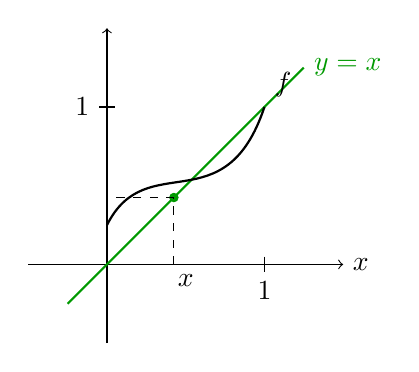
\begin{tikzpicture}
    % Ejes
    \draw[->] (-1,0) -- (3,0) node[right] {$x$};
    \draw[->] (0,-1) -- (0,3);
    % Marcas
    \draw (2,0.1) -- (2,-0.1) node[below] {$1$};
    \draw (0.1,2) -- (-0.1,2) node[left] {$1$};
    \draw (1,0) node[below] {$x$};
    % Funciones
    \draw[thick, green!60!black] (-0.5,-0.5) -- (2.5,2.5) node[right] {$y=x$};
    \draw[thick, black] (0,0.5) .. controls (0.5,1.5) and (1.5,0.5) .. (2,2) node[above right] {$f$};
    % Intersección
    \filldraw[green!60!black] (0.85,0.85) circle (1.5pt);
    \draw[dashed] (0.85,0) -- (0.85,0.85) -- (0,0.85);
\end{tikzpicture}
\end{center}

\textbf{Solución:} Definimos la función $g(x)=f(x)-x$. % [cite: 83]
Podemos suponer sin pérdida de generalidad que $f(0)>0$ y $f(1)<1$, % [cite: 84, 85, 86, 87, 89]
porque si $f(0)=0$ o $f(1)=1$ entonces ya se tiene el resultado. % [cite: 88, 91]
Entonces $g(0)=f(0)-0>0$ y $g(1)=f(1)-1<0$. % [cite: 90, 94]
Por el teorema de Bolzano, existe $x \in [0,1]$ tal que $g(x)=0$, es decir $f(x)=x$. % [cite: 90, 95, 96]
\end{example}

\begin{teorema}[Teorema del valor intermedio (T.V.I)] % [cite: 97]
Supongamos que $f$ es una función real y continua en un intervalo compacto de $\R$. % [cite: 98, 99, 100, 101, 104]
Supongamos que existen dos puntos $\alpha$ y $\beta$ tales que $f(\alpha) \neq f(\beta)$. % [cite: 104, 106]
Entonces $f$ toma todos los valores comprendidos entre $f(\alpha)$ y $f(\beta)$. % [cite: 104, 105, 107, 108]
\end{teorema}

\begin{dem}
Supongamos sin pérdida de generalidad que $f(\alpha) > f(\beta)$. % [cite: 109, 110]
Sea $k \in (f(\beta), f(\alpha))$. % [cite: 110, 113, 114, 118]
Definimos la función $g(x) = f(x) - k$. % [cite: 111, 115, 119]
$g$ es continua en el intervalo comprendido entre $\alpha$ y $\beta$. % [cite: 120, 121, 122, 123, 124, 125]
Notemos que $g(\alpha) = f(\alpha) - k > 0$ y $g(\beta) = f(\beta) - k < 0$. % [cite: 125, 127]
Por el teorema de Bolzano existe $c$ tal que $g(c) = 0$, es decir $f(c) = k$. % [cite: 128, 129, 131, 132]
\end{dem}

\begin{teorema}
Sea $f: X \to Y$ continua y $E \subseteq X$ conexo. Entonces $f(E)$ es conexo. % [cite: 133, 134, 135, 136, 137, 139]
\end{teorema}

\begin{dem}
Supongamos por contradicción que $f(E)$ es disconexo, % [cite: 140, 155]
es decir existen $A$ y $B$ abiertos en $f(E)$ tales que $A \neq \emptyset$, $B \neq \emptyset$, $A \cap B = \emptyset$ y $f(E) = A \cup B$. % [cite: 140, 141, 142, 143, 156]
Sea $G = f^{-1}(A) \cap E$ y $H = f^{-1}(B) \cap E$. % [cite: 145, 157]
Veamos que $G$ y $H$ forman una separación de $E$. % [cite: 146, 147, 158]
Como $f$ es continua, $f^{-1}(A)$ y $f^{-1}(B)$ son abiertos en $E$. % [cite: 148, 159, 163, 167, 168, 169]
Luego $G$ y $H$ son abiertos en $E$. % [cite: 151, 160]

\textbf{Afirmación:} $E \subseteq G \cup H$. % [cite: 161]
En efecto, si $x \in E$, entonces $f(x) \in f(E) \subseteq A \cup B$. % [cite: 162, 170]
Es decir $f(x) \in A$ o $f(x) \in B$. % [cite: 171]
Luego $x \in G$ o $x \in H$. Por lo tanto $E \subseteq G \cup H$. % [cite: 172, 174, 178]
Notemos que $G \cup H \subseteq E$. Por lo anterior, $E = G \cup H$. % [cite: 175, 176, 177, 178]

\textbf{Afirmación:} $G \cap H = \emptyset$. % [cite: 179]
Supongamos que existe $x \in G \cap H$, entonces $x \in G = f^{-1}(A) \cap E$ y $x \in H = f^{-1}(B) \cap E$. % [cite: 180, 181, 183, 184]
Es decir $f(x) \in A \cap B$, lo que es una contradicción porque $A \cap B = \emptyset$. % [cite: 189]

\textbf{Afirmación:} $G \neq \emptyset$ y $H \neq \emptyset$. % [cite: 184, 190]
Como $A \neq \emptyset$ y $A \subseteq f(E)$, entonces $f^{-1}(A) \subseteq G$. % [cite: 185, 186, 193]
Como $B \neq \emptyset$ y $B \subseteq f(E)$, entonces $f^{-1}(B) \subseteq H$. % [cite: 190, 195]

Por lo anterior $G$ y $H$ forman una separación para $E$, es decir $E$ es disconexo. % [cite: 191, 192, 197, 198]
¡Contradicción! pues $E$ es conexo. % [cite: 198, 199]
\end{dem}

\begin{teorema}[Teorema del valor intermedio] % [cite: 200]
Sea $f: [a,b] \to \R$ una función continua. % [cite: 201, 204, 206]
Si $f(a) \neq f(b)$ y $c$ es un número en el intervalo comprendido entre $f(a)$ y $f(b)$, % [cite: 206, 207]
entonces existe $x \in (a,b)$ tal que $f(x) = c$. % [cite: 208]
\end{teorema}

\begin{dem}
Como $f$ es continua entonces $f([a,b])$ es conexo. % [cite: 209, 213]
Supongamos sin pérdida de generalidad que $f(a) < f(b)$. % [cite: 210, 211, 212]
Sea $c \in (f(a), f(b)) \subseteq f([a,b])$, porque $f([a,b]) \subseteq \R$ es conexo. % [cite: 214, 215]
Luego $f([a,b])$ es un intervalo. % [cite: 215, 219]
Por lo anterior, existe $x \in (a,b)$ tal que $f(x) = c$. % [cite: 216, 220]
\end{dem}

\section*{Continuidad uniforme} % [cite: 217]

\begin{remark}
Sea $f: X \to Y$ una función. Supongamos que $f$ es continua en $A \subseteq X$. % [cite: 221, 222, 223, 224, 225]
Si $p \in A$ y $\epsilon > 0$, existe $\delta_{p,\epsilon} > 0$ (depende de $p$ y $\epsilon$) % [cite: 225]
tal que $d_Y(f(p), f(x)) < \epsilon$ si $x \in B_X(p, \delta_{p,\epsilon}) \cap A$. % [cite: 226]
\end{remark}

\begin{definicion}[Continuidad uniforme]
Sea $f: X \to Y$ una función. Entonces decimos que $f$ es uniformemente continua en $A \subseteq X$ si se cumple: % [cite: 227, 228, 233, 234, 235]
Para todo $\epsilon > 0$ existe $\delta_{\epsilon} > 0$ (depende sólo de $\epsilon$) tal que % [cite: 229, 232, 236]
para todo $x, y \in A$ si $d_X(x, y) < \delta_{\epsilon}$ entonces $d_Y(f(x), f(y)) < \epsilon$. % [cite: 230, 231, 237, 238, 239]
\end{definicion}

\begin{remark}
Si $f$ es uniformemente continua en $A$, entonces $f$ es continua en $A$. % [cite: 240, 241, 242, 243, 244, 246, 247, 248]
\end{remark}

\begin{dem}
En efecto, sea $\epsilon > 0$, como $f$ es uniformemente continua en $A$ existe $\delta > 0$ tal que % [cite: 249, 250, 251, 252, 253, 254, 256, 257]
$\forall x,y \in A$ si $d_X(x,y) < \delta$ entonces $d_Y(f(x), f(y)) < \epsilon$. % [cite: 259]
En particular para $y = p$, tenemos que $\forall x \in A$, % [cite: 260, 261, 262, 263]
si $d_X(x,p) < \delta$ entonces $d_Y(f(x), f(p)) < \epsilon$. % [cite: 264]
\end{dem}

\begin{example}
1. La función $f(x) = x$ es uniformemente continua en $\R$. % [cite: 265, 266, 268, 272]
En efecto, sea $\epsilon > 0$, con $\delta = \epsilon$ tenemos que % [cite: 269, 270, 273]
$|f(x) - f(y)| = |x - y| < \delta = \epsilon$. % [cite: 274]

2. La función $f(x) = x^2$ no es uniformemente continua en $\R$. % [cite: 275, 276, 277]
Supongamos que $f$ es uniformemente continua en $\R$. % [cite: 278, 279]
Con $\epsilon = 1$, existe $\delta > 0$ tal que para todo $x, y \in \R$, % [cite: 279]
si $|x - y| < \delta$ implica $|f(x) - f(y)| < 1$. % [cite: 280, 282, 285]
Escogemos $n \in \N$ tal que $n\delta + \delta^2/4 > 1$. % [cite: 281, 283, 286]
En particular para $x = n + \frac{\delta}{2}$ y $y = n$, notemos % [cite: 287, 288]
$|x - y| = n + \frac{\delta}{2} - n = \frac{\delta}{2} < \delta$. % [cite: 289]
Evaluando: $|f(x) - f(y)| = \left| \left(n + \frac{\delta}{2}\right)^2 - n^2 \right| = \left| n^2 + n\delta + \frac{\delta^2}{4} - n^2 \right| = \left| n\delta + \frac{\delta^2}{4} \right|$. % [cite: 290, 291]
$= n\delta + \frac{\delta^2}{4} > 1$. ¡Contradicción! % [cite: 291]
Luego $f$ no es uniformemente continua en $\R$. % [cite: 292]
\end{example}

\begin{remark}
La función $f(x) = x^2$ es continua en $\R$, pero no es uniformemente continua en $\R$. % [cite: 298, 299, 300, 302, 303, 304]
(Ejercicio: leer los ejemplos 1 y 2 en Apostol). % [cite: 293, 294, 295, 296, 297]
\end{remark}

\begin{teorema}[Teorema de Heine] % [cite: 305]
Sea $f: X \to Y$ una función. Sea $A$ un subconjunto compacto de $X$ y supongamos que $f$ es continua en $A$. % [cite: 305, 306, 307, 308, 309, 311, 312, 313]
Entonces $f$ es uniformemente continua en $A$. % [cite: 314, 318, 319, 321]
\end{teorema}

\begin{dem}
Sea $\epsilon > 0$. Como $f$ es continua en $A$, para cada $p \in A$ existe $\delta_p > 0$ % [cite: 315, 316, 317, 320, 322, 326]
tal que si $x \in B_X(p, \delta_p) \cap A$ implica $d_Y(f(p), f(x)) < \frac{\epsilon}{2}$. % [cite: 323, 328]
El cubrimiento $\mathcal{C} = \left\{ B_X\left(p, \frac{\delta_p}{2}\right) \mid p \in A \right\}$ es un cubrimiento abierto de $A$. % [cite: 324, 325, 327, 329]
Luego $A \subseteq \bigcup_{p \in A} B_X\left(p, \frac{\delta_p}{2}\right)$. % [cite: 330, 331]
Como $A$ es compacto, existen $p_1, p_2, \dots, p_k \in A$ tales que % [cite: 332, 333, 334, 335, 337]
$A \subseteq \bigcup_{i=1}^k B_X\left(p_i, \frac{\delta_{p_i}}{2}\right)$. % [cite: 338]
Sea $\delta = \min \left\{ \frac{\delta_{p_i}}{2} \mid i = 1, \dots, k \right\}$. % [cite: 336, 339]
Sean $x, y \in A$ tales que $d_X(x, y) < \delta$. % [cite: 340]
Como $x \in A \subseteq \bigcup_{i=1}^k B_X\left(p_i, \frac{\delta_{p_i}}{2}\right)$, existe $j \in \{1, \dots, k\}$ tal que $x \in B_X\left(p_j, \frac{\delta_{p_j}}{2}\right)$. % [cite: 341, 342]
Veamos que $y \in B_X(p_j, \delta_{p_j})$. % [cite: 343]
En efecto, $d_X(y, p_j) \le d_X(y, x) + d_X(x, p_j) < \delta + \frac{\delta_{p_j}}{2} \le \frac{\delta_{p_j}}{2} + \frac{\delta_{p_j}}{2} = \delta_{p_j}$. % [cite: 344, 345]

\textbf{Afirmación:} $d_Y(f(x), f(y)) < \epsilon$. % [cite: 346]
En efecto, $d_Y(f(x), f(y)) \le d_Y(f(x), f(p_j)) + d_Y(f(y), f(p_j))$. % [cite: 347, 348]
Por la continuidad de $f$ en $p_j$, tenemos que la suma es $< \frac{\epsilon}{2} + \frac{\epsilon}{2} = \epsilon$. % [cite: 349, 350, 351]
\end{dem}

\begin{definicion} % [cite: 352]
Sea $f: X \to X$ una función de un espacio métrico en sí mismo. % [cite: 353, 354, 360, 361]
1. Un punto $p \in X$ es un punto fijo de $f$ si $f(p) = p$. % [cite: 355, 362, 363, 364]
2. La función $f$ se denomina contracción de $X$ si existe un número $0 < \alpha < 1$ % [cite: 356, 357, 358, 359, 365, 366, 367]
($\alpha$ se llama la constante de contracción o coeficiente de contracción) % [cite: 368, 369, 370]
tal que $d(f(x), f(y)) \le \alpha d(x, y)$ para todo $x, y \in X$. % [cite: 371]
\end{definicion}

\begin{example}
La función $f(x) = \frac{1}{2}x$ de $\R$ en $\R$ es una contracción. % [cite: 372, 373, 374, 375, 376]
$|f(x) - f(y)| = \left| \frac{1}{2}x - \frac{1}{2}y \right| = \frac{1}{2}|x - y|$. % [cite: 377]
\end{example}

\begin{remark}
Si $f: X \to X$ es una contracción, entonces $f$ es uniformemente continua en $X$. % [cite: 377, 378, 379, 380]
En efecto, sea $\epsilon > 0$, existe $\delta = \frac{\epsilon}{\alpha}$ tal que % [cite: 381, 382]
si $d(x, y) < \delta$ implica que $d(f(x), f(y)) \le \alpha d(x, y) < \alpha \delta = \alpha \left(\frac{\epsilon}{\alpha}\right) = \epsilon$. % [cite: 383, 384]
\end{remark}

\begin{teorema}[Teorema del punto fijo] % [cite: 385]
Sea $f: X \to X$ una contracción en un espacio métrico completo $X$. % [cite: 385, 386, 387, 390, 392, 393]
Entonces existe un único punto $p \in X$ tal que $f(p) = p$. % [cite: 388, 389, 394]
\end{teorema}

\begin{dem}
\textbf{Unicidad:} Veamos la unicidad. Supongamos que $p$ y $p'$ son puntos fijos de $f$, % [cite: 395, 396, 397, 399]
es decir $f(p) = p$ y $f(p') = p'$. % [cite: 398, 400, 401, 402]
Como $f$ es una contracción, existe $\alpha \in (0, 1)$ tal que % [cite: 403, 404]
$d(f(x), f(y)) \le \alpha d(x, y)$ para todo $x, y \in X$. % [cite: 405]
En particular, con $p$ y $p'$ tenemos: % [cite: 406]
$d(p, p') = d(f(p), f(p')) \le \alpha d(p, p')$. % [cite: 407]
Luego, $d(p, p') \le \alpha d(p, p')$, lo que implica $d(p, p')[1 - \alpha] \le 0$. % [cite: 408, 409]
Pero $1 - \alpha > 0$. % [cite: 411, 412]
Por lo tanto $d(p, p') \le 0$. Pero por definición de métrica $d(p, p') \ge 0$. % [cite: 413]
Luego $d(p, p') = 0$, por lo tanto $p = p'$. % [cite: 414]

\textbf{Existencia:} Para probar la existencia de un punto fijo, sea $x \in X$. % [cite: 415, 416, 417]
Consideremos la siguiente sucesión $\{p_n\}_{n=0}^{\infty} \subseteq X$ que se define recurrentemente como: % [cite: 418, 422, 424, 426, 432]
$p_0 = x$, $p_1 = f(x) = f(p_0)$, $p_2 = f(f(x)) = f(p_1)$, y en general $p_{n+1} = f(p_n)$. % [cite: 419, 420, 421, 423, 427, 428, 430, 431]

\textbf{Afirmación:} $\{p_n\}_{n=0}^{\infty}$ es de Cauchy. % [cite: 429]
En efecto, notemos: % [cite: 433]
$d(p_{n+1}, p_n) = d(f(p_n), f(p_{n-1})) \le \alpha d(p_n, p_{n-1})$ % [cite: 434]
$= \alpha d(f(p_{n-1}), f(p_{n-2})) \le \alpha^2 d(p_{n-1}, p_{n-2})$ % [cite: 435, 436]
$= \alpha^2 d(f(p_{n-2}), f(p_{n-3})) \le \alpha^3 d(p_{n-2}, p_{n-3})$ % [cite: 437, 438, 440]
Continuando así, obtenemos $\dots \le \alpha^n d(p_1, p_0)$. % [cite: 441]
Por lo anterior, $d(p_{n+1}, p_n) \le \alpha^n d(p_1, p_0) = \alpha^n c$ (llamando $c = d(p_1, p_0)$). % [cite: 442]

Para $m > n$, usando la desigualdad triangular en cada paso tenemos: % [cite: 443, 444, 445]
$d(p_m, p_n) \le d(p_m, p_{m-1}) + \dots + d(p_{n+1}, p_n)$ % [cite: 446, 447]
$\le \sum_{k=n}^{m-1} d(p_{k+1}, p_k) \le \sum_{k=n}^{m-1} \alpha^k c = c \frac{\alpha^n - \alpha^m}{1 - \alpha} \le \frac{c \alpha^n}{1 - \alpha}$. % [cite: 439, 448]

Como $0 < \alpha < 1$, al hacer $n \to \infty$, $\alpha^n \to 0$. Luego la sucesión es de Cauchy.
Como $X$ es completo, la sucesión converge a un punto $p \in X$.
Como $f$ es una contracción, es continua, por lo que $f(p) = f(\lim_{n \to \infty} p_n) = \lim_{n \to \infty} f(p_n) = \lim_{n \to \infty} p_{n+1} = p$.
Luego $p$ es un punto fijo de $f$. % [cite: 449, 450, 451, 452]
\end{dem}